\documentclass[cn,11pt]{elegantbook}




%插入图片包
\usepackage[graphicx]{realboxes}
\usepackage{subfigure}
\usepackage{float}









 \newcommand\degree{^\circ} %使用未定义的的命令的时候需要定义

% 修改标题页的橙色带
\definecolor{customcolor}{RGB}{32,178,170}
\colorlet{coverlinecolor}{customcolor}
\usepackage{cprotect}






\title{言为何语}
\author{S.K.}
\date{\today}
\institute{蹈微}
\cover{1.jpg}








\begin{document}

\maketitle%输出标题
\frontmatter
\tableofcontents%命令输出论文目录
\mainmatter


\chapter{编程语言}

学习一门新的语言总会是不容易的。

\section{学习latex日记}
  
当 latex 处理源文件时, 首先需要知道的就是作者所要创建的文档类型,即
\href{https://zhuanlan.zhihu.com/p/247888156}{\underline{documentclass}}。


关于图形的绘制,我们一般使用
\href{https://zhuanlan.zhihu.com/p/48300815}{\underline{TikZ}}
来在latex中作画。
\href{http://cremeronline.com/LaTeX/minimaltikz.pdf}{\underline{minimaltikz.pdf}}just like a little teaching.
里面从开始讲到了坐标制图。
 理论上讲,any things can draw out by this one.


\subsection{examples}

勾股定理可以用现代语言表述如下:
直角三角形斜边的平方等于两腰的平方和。
可以用符号表示为:设直角三角形$ABC$,其中

$\angle C=90\degree$,则有 % \degree没被定义的话需要定义

\begin{equation} %equation用来引入带编号的公式
AB^2=BC^2+AC^2
\end{equation}



      
\begin{lstlisting}
关于目录和标题的建立, 
可以用'\tableofcontents'生成目录,编译两次就可以生成。
\section{一级标题}
\subsection{二级标题} 
\subsubsection{三级标题}

关于反斜杠,可以用`\backslash'输入。
\end{lstlisting}

关于数学常用符号:

some webs in wild:  
\href{https://blog.csdn.net/Motarookie/article/details/124024409}{\underline{web1}}
\href{https://zhuanlan.zhihu.com/p/95886235}{\underline{web2}}




\subsection{ 插入图片}

参照\href{https://blog.csdn.net/panbaoran913/article/details/122849294?spm=1001.2101.3001.6650.1&utm_medium=distribute.pc\_relevant.none-task-blog-2}
{\underline{latex 插入图片}},we have done the below things.
    
\begin{figure}[H]%%图,[htbp]是浮动格式
\centering
\subfigure{
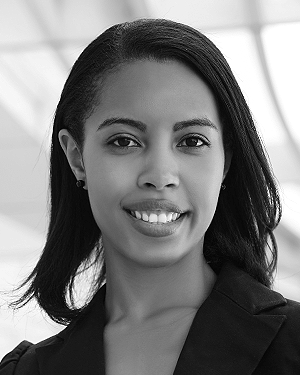
\includegraphics[width=2.5cm,height=2.5cm]{./a1.png} 
}
\hspace{2mm}
\subfigure{
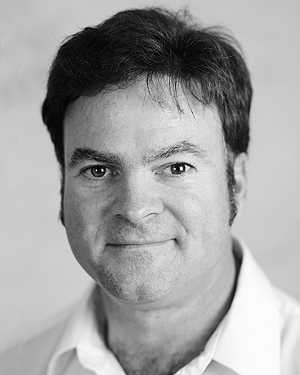
\includegraphics[width=2.5cm,height=2.5cm]{./a2.png} 
}
\caption{man and woman}
\end{figure}


\begin{lstlisting}
    删除线需要调用package:
    \usepackage{ulem}
    而后是:
    \sout{文字} %删除线
    \uwave{文字} %波浪线
    \xout{文字} %斜删除线
    \uuline{文字}  %双下划线
\end{lstlisting}



\chapter{学习C语言日记}
      
\href{https://sourceforge.net/projects/mingw-w64/}{\underline{编译器下载网站}}

        

\begin{lstlisting}
#include <stdio.h>
int main()
{ 
printf("hello world\n");
return 0;
}

\end{lstlisting}





\chapter{单片机学习}

\subsection{流水灯}
\begin{lstlisting}

//流水灯
#include "reg52.h"
#include "intrins.h"
#define LED_PORT P2 
typedef unsigned int u16; 
typedef unsigned char u8;

void delay_10us(u16 ten_us)
	{
	while(ten_us--);
}


void main()
{
u8 i=0;
LED_PORT=~0x01;
 delay_10us(50000);
while(1)
{
for(i=0;i<7;i++) 
{
LED_PORT=_crol_(LED_PORT,2);
delay_10us(50000);
}
for(i=0;i<7;i++) 
{

\end{lstlisting}

\subsection{蜂鸣器}
\begin{lstlisting}
    //蜂鸣器

    #include "reg52.h"
    
    typedef unsigned int u16; //对系统默认数据类型进行重定义
    typedef unsigned char u8;
    
    sbit BEEP=P2^5; //将 P2.5 管脚定义为 BEEP
    
    void delay_10us(u16 ten_us)
    {
    while(ten_us--);
    }
    
    void main()
    {
    u16    i=2000;
    while(1)
    {
    while(i--)//循环 2000 次
    {
    BEEP=!BEEP;//产生一定频率的脉冲信号
    delay_10us(100);
    }
    
    i=0;//清零
    BEEP=0;//关闭蜂鸣器
    }
    }
    
    
\end{lstlisting}

\subsection{数码管}

\begin{lstlisting}

    //数码管

    #include "reg52.h"
    typedef unsigned int u16; //对系统默认数据类型进行重定义
    typedef unsigned char u8;
    
    #define SMG_A_DP_PORT P0 //使用宏定义数码管段码口
    //共阴极数码管显示 0~F 的段码数据
    u8 gsmg_code[17]={0x3f,0x06,0x5b,0x4f,0x66,0x6d,0x7d,0x07,
    0x7f,0x6f,0x77,0x7c,0x39,0x5e,0x79,0x71};
    
    void main()
    {
    SMG_A_DP_PORT=gsmg_code[0];//将数组第 1 个数据赋值给数码管段选口
    while(1)
    {
    }
    }
    
    
\end{lstlisting}



\subsection{动态数码管}

\begin{lstlisting}
    //动态数码管

    #include "reg52.h"
    typedef unsigned int u16;//对系统默认数据类型进行重定义
    typedef unsigned char u8;
    #define SMG_A_DP_PORT P0 //使用宏定义数码管段码口
    
    //定义数码管位选信号控制脚
    sbit LSA=P2^2;
    sbit LSB=P2^3;
    sbit LSC=P2^4;
    //共阴极数码管显示 0~F 的段码数据
    u8  gsmg_code[17]={0x3f,0x06,0x5b,0x4f,0x66,0x6d,0x7d,0x07,
                0x7f,0x6f,0x77,0x7c,0x39,0x5e,0x79,0x71};
                
    void delay_10us(u16 ten_us)
    {
    while(ten_us--);
    }
    
    void smg_display(void)
    {
    u8 i=0;
    for(i=0;i<8;i++)
    {
    switch(i)//??
    {
    case 0: LSC=1;LSB=1;LSA=1;break;
    case 1: LSC=1;LSB=1;LSA=0;break;
    case 2: LSC=1;LSB=0;LSA=1;break;
    case 3: LSC=1;LSB=0;LSA=0;break;
    case 4: LSC=0;LSB=1;LSA=1;break;
    case 5: LSC=0;LSB=1;LSA=0;break;
    case 6: LSC=0;LSB=0;LSA=1;break;
    case 7: LSC=0;LSB=0;LSA=0;break;
    }
    SMG_A_DP_PORT=gsmg_code[i];//传送段选数据
    delay_10us(100);//延时一段时间,等待显示稳定
    SMG_A_DP_PORT=0x00;//消音
    }
    }
    
    void main()
    {
    while(1)
    {
    smg_display();
    }
    }
    
    

\end{lstlisting}



























\chapter{数学语言}
是天使还是恶魔?


\section{卷积}


序列卷积运算:
\begin{equation}
y[k]=x_1[k]*x_2[k] =\sum_{n=-\infty}^{\infty}x_1[n]x_2[k-n]
\end{equation}

互相关运算:
\begin{equation}
r_{xy}[k] = \sum_{k=-\infty}^{\infty} x[n]y[n+k]
%定义式
          = \sum_{k=-\infty}^{\infty} x[-(k-n)]y[n]
          = x[-k]*y[k]
%  n=(-(k-n))+k
\end{equation}

自相关函数:
\begin{equation}
r_{x}[k] = \sum_{k=-\infty}^{\infty} x[n]x[k+n]
\end{equation}

\section{积分练习}
       
常见泰勒公式:
   \begin{equation}
    e^x =1 + x + \frac{x^2}{2!}  
    +  \cdot \cdot \cdot  
    +\frac{x^n}{n!} 
    +o(x^n) 
   \end{equation}

   \begin{equation}
    sinx = x - \frac{x^3}{3!} 
    + \cdot \cdot \cdot  
    + (-1)^{n-1} \frac{x^{2n-1}}{(2n-1)!} 
    + o(x^{2n-1})
   \end{equation}

   \begin{equation}
       cosx = 1- \frac{x^2}{2!} 
       + \cdot \cdot \cdot 
       + (-1)^n \frac{x^{2n}}{(2n)!}
       + o(x^{2n})
   \end{equation}

   \begin{equation}
       ln(1+x) = x - \frac{x^2}{2}
       +\cdot \cdot \cdot
       +(-1)^{n-1}\frac{x^n}{n}
       +o(x^n)
   \end{equation}

   \begin{equation}
       (1+x)^\alpha = 1 + \alpha x 
       + \frac{\alpha(\alpha-1)}{2!}x^2
       + \cdot \cdot \cdot
       + \frac{\alpha(\alpha-1) \cdot \cdot \cdot(\alpha-n+1)}{n!}x^n
       + o(x^n) 
   \end{equation}

   

\section{误差}
       

      


\chapter{物理模型}
  积木,还是武器?

\section{电磁学}

        
\appendix
\chapter{自然资料}



\end{document}
